\subsection{Hall Sensor}
There are two hall sensors implemented on the vehicle, one on each belt, at the front gear (See \figref{vehicleDescriptionDriveTrain} in \secref{})\todo{Make the sec ref}. A hall sensor is a sensor that is activated when exposed to a magnetic field. The sensors are placed beside the front wheels, on which there are four magnets, placed so that there is a quarter of a turn between them. The hall sensor is illustrated on \figref{HallSensor}.

 \begin{figure}[H]
	\centering
	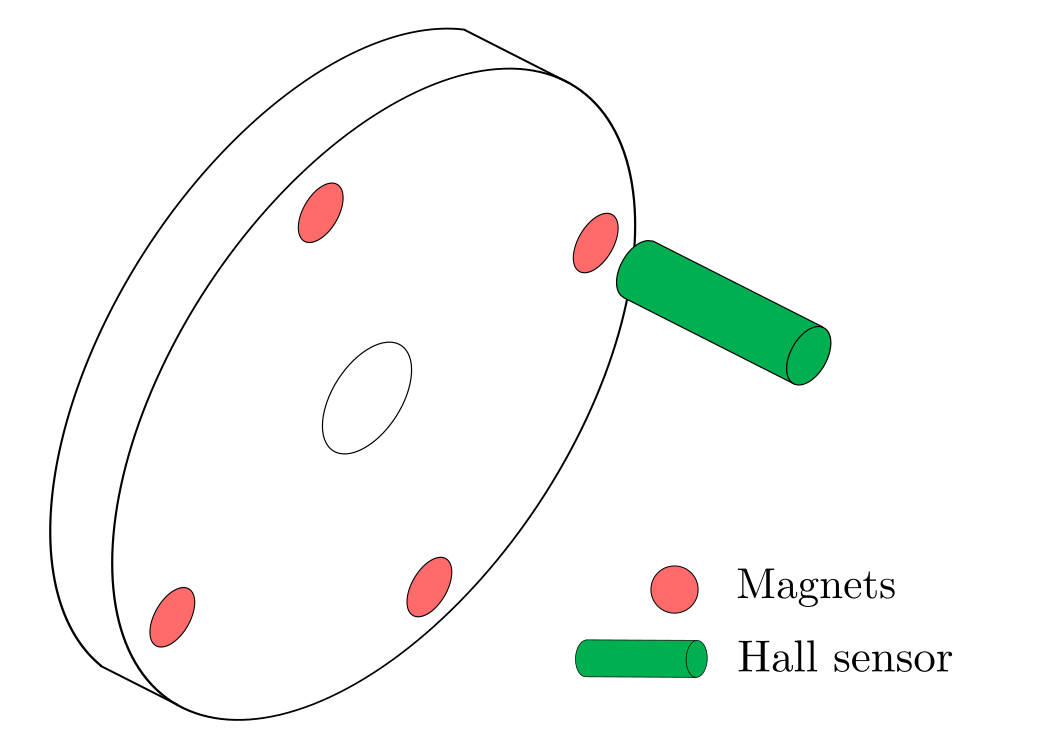
\includegraphics[scale=0.5]{figures/HallSensor3D.pdf}
	\caption{Illustration of the hall sensor.}
	\label{HallSensor}
\end{figure}

The Hall sensor will give a voltage output each time one of the magnets is in front of the hall sensor. This will give a signal each quarter of a turn of the wheel. As the distance between each magnets is not the same, the calculations will be taken for each magnets independently.
Knowing the time a turn of the wheel will take by measuring the time between four outputs, and the distance that the vehicle travels on that time, the speed of the vehicle can be calculated.

When the vehicle is starting to move, the first turn of the wheel can not be used because four signals must be registred to calculate the speed. Therefore the speed can only be calculated by the first output of the second turn.\\\\

The two hall sensors are used for keeping track of the speed of each belt because the belts run at different speeds when the vehicle is turning, which is controled by the servo.
